\documentclass[a4paper, 11pt]{article}
\usepackage{listings}
\usepackage{amsmath}
\newcommand{\argmax}{\operatornamewithlimits{arg\,max}}
\newcommand{\argmin}{\operatornamewithlimits{arg\,min}}
\lstset{
	tabsize=2,
	basicstyle=\footnotesize\ttfamily,
	language = Java,
	keywordstyle =\bfseries \color{blue},
	commentstyle =\color{green},
	stringstyle =\itshape \color{red}
}
\usepackage{graphicx}
\usepackage[
	colorlinks=true,
	urlcolor=black,
	linkcolor=blue,
	citecolor = black,
	naturalnames=true,
	pdftitle={Graph Clustering and Visualization Framework},
	pdfsubject={Manual},
	pdfauthor={R. Speck},
	pdfkeywords={BorderFlow, CUGAR, visualization, graph, cluster }
]{hyperref}

\begin{document}
\thispagestyle{empty}

\begin{titlepage}
\begin{center}

\textsc{\LARGE CUGAR \Large - Graph Clustering and Visualization Framework}\\[1.5cm]
\textsc{\Large} University of Leipzig\\[0.5cm]

\begin{minipage}{0.7\textwidth}
	\begin{flushleft} 
		\large
		\emph{Contributors:}\\
		R. Speck\\
		A.-C. Ngonga Ngomo
	\end{flushleft}
\end{minipage}\\
[2cm]
\begin{figure}[h!]
	\centering
	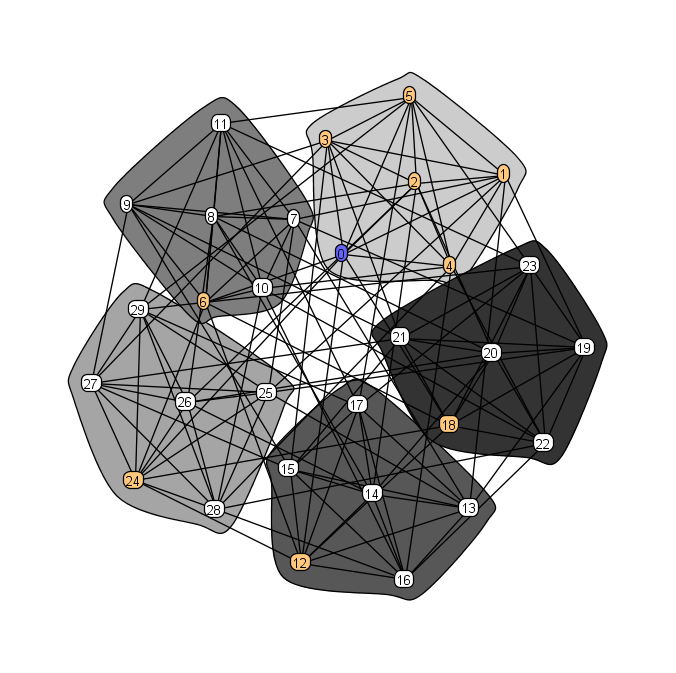
\includegraphics[height=10cm]{img/clique.png}
	\caption{A clustered 6-5-partite clique.}
	\label{fig:clique}
\end{figure}
\vfill

{\large \today}
\end{center}
\end{titlepage}
\tableofcontents

\newpage
\section{Introduction}
	This manual is intended as a guide for using the Graph Clustering and Visualization Framework (CUGAR), 
	a tool and framework for graph clustering. It presents the functionality of CUGAR in its current version. 
	In addition, it provides insight in the architecture of the underlying framework, so as to enable any user 
	to extend it as required for his purposes.
	\subsection{Purpose}
		Our main aim while developing CUGAR was to provide a lightweight framework that allows rapid integration 
		and testing of novel graph clustering algorithms. Roughly speaking, CUGAR in its current version allows to 
		(1) visualize input graphs stored in several formats, 
		(2) cluster the input graph using any of the algorithms integrated, 
		(3) integrate novel algorithms very efficiently as required (section \ref{sec:cvk.cluster}), 
		(4) explore the resulting clustering and 
		(5) store the resulting clustering for further processing.

		The toolkit is intended for both beginners and experts: CUGAR provides an easy-to-use graphical interface 
		for users that not yet familiar with graph clustering. In addition, CUGAR's modular architecture allows the 
		rapid integration of new clustering algorithms. Ergo, experts are provided with means to 
		(1) efficiently develop, 
		(2) visualize the results and 
		(3) evaluate the quality of (new) clustering algorithms for graphs. 
		The user interface was designed to be as intuitive as possible, so as to allow the easy manipulation of 
		nodes and clusters during the exploration of the input graph and resulting clustering. In addition, the 
		tool implements several metrics that provide a numeric impression of the quality of the clustering 
		achieved by the algorithm applied. 

		The visualization component is based on the prefuse visualization toolkit\footnote{\url{http://prefuse.org}}, 
		graphs automatically generated by graph models based among others on the jung framework
		\footnote{\url{http://jung.sourceforge.net}} and the Lucene search 
		engine\footnote{See \url{http://lucene.apache.org/java/1\_4\_3} for all options.}, that 
		supports a fast search over nodes. 
		CUGAR implements the clustering algorithms Affinity Propagation, BorderFlow, Chinese Whispers, k-Nearest Neighbours 
		and MCL in its current version. Further algorithms will be integrated soon. 
		CUGAR is open-source and available under the BSD License.

	\subsection{Requirements}
		The only requirement to run the application is an installed 
		JRE\footnote{\url{http://www.java.com/de/download/manual.jsp}} version 1.6 upwards. 
\newpage
\section{Using CUGAR}
	\subsection{Launching}
		To start the application, double-click the cugar.jar file or type the following in your terminal: 
		\textit{java -jar cugar.jar}.
		Should you get \textit{Out of Memory errors}, increase the maximum heap size for your java virtual machine 
		(JVM) via the \textit{-Xmx} option\footnote{\url{http://java.sun.com/docs/hotspot/gc5.0/gc_tuning_5.html}}.

		After you have started the application, you should see the main panel as shown in figure below.
		
		\begin{figure}[ht!]
			\centering
			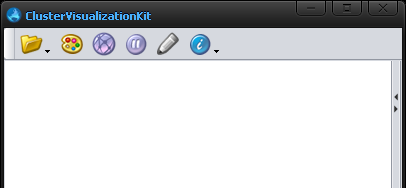
\includegraphics[width = 0.7\textwidth]{img/start.png}
			\caption{Welcome screen}
			\label{fig:start}
		\end{figure}

	\subsection{Loading data}
		The first step in using the application is to read data. Two types of data can be loaded into CUGAR: 
		user-generated data (i.e., a file) or automatically generated data for tests purposes. 

	\subsubsection{Loading user-generated data} \label{sec:openfile}
		Currently, the CUGAR supports delimiter separated text files and the XML-format GraphML as input format for user-generated data.  
		To import such data, use the toolbar or the corresponding keyboard shortcut as displayed in figure \ref{fig:toolbar}. 
		After you have selected ``Open File'' from toolbar menu, you will see the dialog shown in \ref{fig:openfile}. 
		By using this dialog, you can choose the type of files to import, i.e., whether a delimiter separated or a GraphML file should be imported. 
		The default ``Open File'' dialog is set to import delimiter separated data files as they are more commonly used than GraphML. 
		The file extension is used to determine the file delimiter (\ref{sec:delimiterFiles}).
		
		\begin{figure}[h!]
		\centering 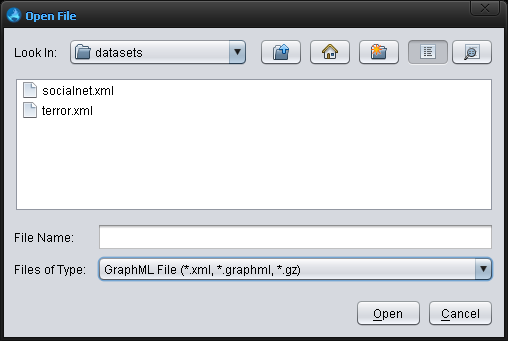
\includegraphics[width = 0.6\textwidth]{img/openfile.png}
		\caption{Open File Dialog}\label{fig:openfile}
		\end{figure}

	\subsubsection{Loading automatically generated data} \label{sec:opengraph}
		This menu item allows you to load automatically generated data instead of user-generated data. 
		The basic intention behind this feature was to allow users to view the results of algorithms on 
		small graphs without having to encode a graph manually.\\ 
		After selecting ``Open Graph'', you will see the submenu as shown in figure \ref{fig:toolbar}. 
		This submenu allows you to choose from various types of graphs to load, including the a topped tetrahedron,  
		random $n$-$k$ partite cliques (i.e., graphs that contains $k$ cliques of $n$ nodes, with 
		$3 \leq n \leq 15$, $2 \leq k \leq 14$ and $k \le n$), 
		graphs generated by using the binomial model of Erd\H{o}s and R\'{e}nyi (n=200, p = 2.4/n) and some others 
		that comes from the prefuse and jung library.
		
		\begin{figure}[ht!]
		\centering 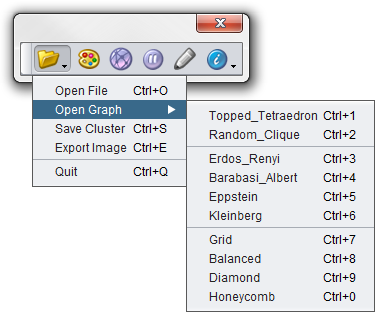
\includegraphics[width = 0.5\textwidth]{img/toolbar.png}
		\caption{CURAR's toolbar}\label{fig:toolbar}
		\end{figure}
		
	\subsection{Configuring}
		\begin{figure}[h!]
			\centering 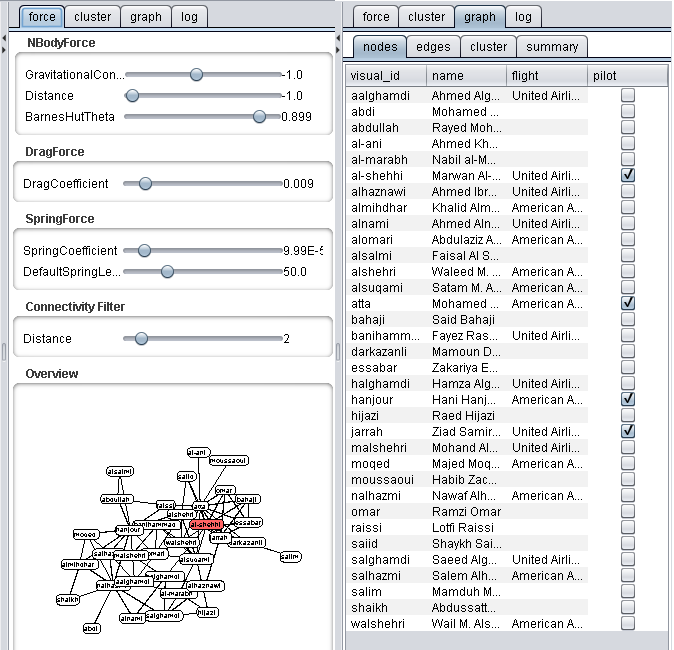
\includegraphics[width = 1\textwidth]{img/settings.png}
			\caption{Force configurations (left) and clickable node table (right).} \label{fig:force}
		\end{figure}
		
		After you have loaded your data, you may want to configure the force layout to display your graph in a 
		fashion suitable to your taste. To achieve this, use the sliders (figure \ref{fig:force} - left) in the 
		three boxes NBodyForce, DragForce and SpringForce. You can also change the Connectivity Filter, this 
		entry controls the maximal distance between nodes that are displayed and the node that is currently selected. 
		Obviously, pushing this value to more than 3 when a large graph is loaded might lead to longer processing 
		time before a stable graph is displayed. To stop the animation, please use the ``Play/Pause'' button on the menu bar.
		%need to comment the overview picture. That would help users.

		One of the drawback of displaying nodes based on the surroundings of the node that is currently selected 
		is that nodes that are at an infinite distance (i.e., not connected) of the currently selected node never 
		get displayed. To guarantee that the user retains an overview of the graph, the interface provide an overview window below the sliders.
		To ensure that all nodes are displayed, we added the grid button that allows to display all nodes are once. 
		Another way to select a node and thus to display the surroundings of the node is to use the clickable nodes table (figure \ref{fig:force} - right)
		or to select all nodes in a cluster use the clickable cluster table.		
	
	\subsection{Clustering}	
		\begin{figure}[h!]
			\centering 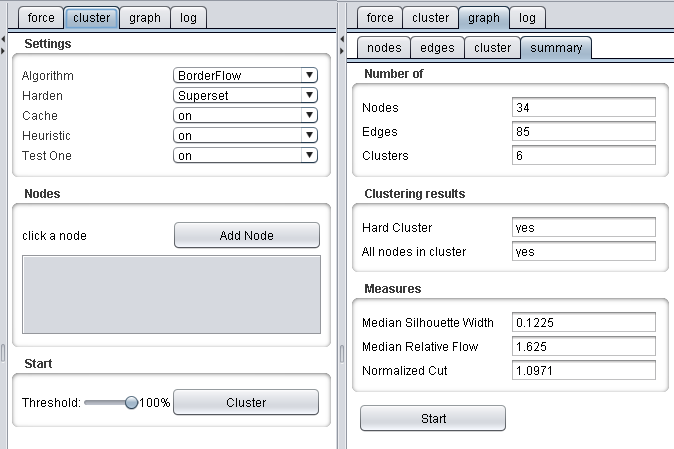
\includegraphics[width = 1\textwidth]{img/summary.png}
			\caption{Clustering configurations (left) and graph statistic (right).}	\label{fig:summary}
		\end{figure}
		
		The main aim of the CUGAR is to enable users to test clustering approaches. 
		To choose a clustering algorithm to process the data you loaded, go to the cluster tab (figure \ref{fig:summary} - left), 
		pick one of the algorithms (section \ref{sec:algo}) from the ``Settings'' box and select/set the parameters you need for your clustering process. 
		CUGAR was designed in such a way that each algorithm has its own clustering configuration. 
		For example, the BorderFlow and k-Nearest Neighbours algorithms allow to select the nodes that are used as seed for clustering; 
		they also provide a threshold slider, which sets the percentage of the maximal connectivity that a node can maximally have to be used as seed 
		(obviously, moving the slider to 0 causes all nodes to be used as seeds).
		The threshold slider for Chinese Whispers sets the percentage of the maximal edge weight.
		After having configured your clustering algorithm, press the ``Cluster'' button to start the clustering process. 
		Depending on the size of the input data and the algorithm, the clustering might take a while. Please be patient. 

		After the completion of the clustering, CUGAR allows you to navigate through the clusters by using mouse actions on the main panel. 
		By using the color button, you can turn the display of the clusters to greyscale or color. 
		Finally, the ``Save clusters'' menu item under the folder icon allows to save the results of the clustering for further processing or evaluation.

\section{Supported data formats} \label{sec:files}
	CUGAR supports various file formats, which are explained below. 
	Furthermore, it is possible to open such graphs directly from the menu bar in the application as described in section \ref{sec:opengraph}. 
	The use of edge weights is possible in all file types. If no weights are set, the weight value is set to 1. 
	Because most clustering algorithms are defined in such a way that they do not support edges that begin and end at the same node, 
	edges with the same node as source and target are ignored when reading the input data. In addition, nodes without edges are ignored.

	\subsection{GraphML/XML}
		GraphML is a XML format supporting graph structure and typed data schemas for both nodes and edges.
		For more information about this format, see the GraphML home page\footnote{\url{http://graphml.graphdrawing.org/}}. 
		The only restriction of CUGAR when reading GraphML is that it does not support the mix of weighted and unweighted edges within one graph. 

	\subsection{CSV/SSV/Tab/Txt} \label{sec:delimiterFiles}
		CUGAR supports an edge list file format in which each line is an edge. 
		In a line the first term is a source node, second term is a target node and the last term is a weight. 
		We use delimiter separated values, each term in a line has to be separated dependents
		on the used file format extension as shown in the following table.

	\begin{center}
		\begin{tabular}[ht]{|l|l|}
		\hline
		File Extension & Separator\\
		\hline
		csv & comma \\
		ssv & space\\
		tab/txt & tabulator \\
		\hline
		\end{tabular}
	\end{center}

\newpage
\section{Supported algorithms} \label{sec:algo}
	CUGAR is intended to enable beginners to utilize exisiting algorithms and developers to test their new algorithms. 
	The current version of CUGAR implements the clustering algorithms described in the following.

	\subsection{Affinity Propagation} \label{sec:ap}
		Affinity Propagation takes as input measures of similarity between pairs of data points \cite{ap}. 
		Real-valued messages are exchanged between data points until a high-quality set of exemplars and corresponding clusters
		gradually emerges. %Affinity propagation found clusters with much lower error than
		%other methods, and it did so in less than one-hundredth the amount of time.

	\subsection{BorderFlow} \label{sec:bf}
		BorderFlow is a general-purpose graph clustering algorithm \cite{4}. 
		It uses solely local information for clustering and achieves a soft clustering of the input graph. 
		The standard definition of clusters is that they have a maximal intra-cluster density and inter-cluster sparseness. 
		When considering a graph as the description of a flow system, this definition of a cluster implies that a cluster X 
		can be understood as a set of nodes such that the flow within X is maximal while the flow from X to the outside is minimal. 
		The idea behind BorderFlow is to maximize the flow from the border of each cluster to its inner nodes (i.e., the nodes within the cluster) 
		while minimizing the flow from the cluster to the nodes outside of the cluster.
		
	\subsection{Chinese Whispers} \label{sec:cw}
		Chinese Whispers is a randomized graph-clustering algorithm, which is time-linear in the number of edges \cite{Bie06a}.
		Intuitively, the algorithm works as follows in a bottom-up fashion: First, all nodes get different
		classes. Then the nodes are processed for a small number of iterations and inherit the strongest class
		in the local neighborhood. This is the class whose sum of edge weights to the current node is
		maximal. In case of multiple strongest classes, one is chosen randomly. Regions of the same class
		stabilize during the iteration and grow until they reach the border of a stable region of another class.
		Note that classes are updated immediately: a node can obtain classes from the neighborhood that were
		introduced there in the same iteration.
	
	\subsection{k-Nearest Neighbours} \label{sec:knn}
		In pattern recognition, the k-nearest neighbours algorithm (k-NN) was orginally a method
		for classifying objects based on closest training examples in the feature space. 
		k-NN is a type of instance-based learning, or lazy learning where the function is only approximated locally and all 
		computation is deferred until classification. An object is classified by a majority vote of its neighbors, 
		with the object being assigned to the class most common amongst its k nearest neighbors (k is a positive integer, typically small). 
		If k = 1, then the object is simply assigned to the class of its nearest neighbor. 
		k-NN can be used for seed-based clustering simply by stating that each of the $k-1$ nearest neighbors of an input seed 
		are the elements of a cluster of size $k$ (seed + neighbors). 
		Clusters that happen to containe the same elements are merged to one cluster.
	
	\subsection{MCL} \label{sec:mcl}
		The basic idea underlying the MCL algorithm \cite{5} is that dense regions (i.e., clusters) in sparse graphs correspond 
		with regions in which the number of $k$-length paths is relatively large. 
		Thus, random walks of length $k$ have a higher probability to begin and end in the same dense region than for other paths. 
		The algorithm starts uses a stochastic matrix $M$ to represent the input graph. 
		Then, it alternates two operations (expansion and inflation) to compute the set of transition probabilities until 
		$M$ does not change substantially. The result is a complete and does not contain overlapping clusters. 

\section{Measurements} \label{sec:mes}
	Several means for assessing the quality of a clustering have been defined in the past.
	In this section, we describe those measurements that are computed after the completion of each clustering (figure \ref{fig:summary} - right). 
	These metrics can be easily extended as required by the user. 
	In the following, we will assume that $G = (V, E, \omega)$ is a weighted directed graph with a set of vertices $V$, 
	a set of edges $E$ and a weighing function $\omega$, which assigns a positive weight to each edge $e \in E$.
	$V$ can be partitioned into $k$ subsets $X_{1},...,X_{k}$.
	Furthermore, we define $\Omega(X_{1},X_{2}) = \sum_{x_{1} \in X_{1}, x_{2} \in X_{2}} \omega(x_{1}x_{2})$ as
	the function that assigns the total weight of the edges from a subset $X_{1} \subset V$ to a subset $X_{2} \subset V$.
	
	The toolkit implements the median of average silhouette width, the median of the relative flow and the normalized cut measures.

	\subsection{Median of average silhouette width}
		The silhouette measures of a set is given by the following equation\cite{1}
		\[
		s(x) = \frac{b(x) - a(x)}{max\{a(x),b(x)\}}
		\]
		where $a(x)$ is the average similarity between vertex $x\in X$
		and all other vertices in subset $X$,
		and $b(x)$ is the average similarity between vertex $x\in X$ and
		all other vertices in the neighbour subsets to $X$.\\
		%The average of $s(x)$ for all vertices $x$ in a subset $X$, is called
		%the average silhouette width of $X$.
		%The average $\overline s$ of $s(x)$ for all vertices $x\in V$, is called
		%the average silhouette width for the entire data set.\\
		%''The Silhouette Coefficient(SC) is a measure where the maximum is taken over all k for which the silhouettes can be
		%constructed[...]''\cite{0}.
		%\[
		%SC = max_{k} \overline s(k)
		%\]
		%Values between 0.7 and 1.0 indicate clustering results with excellent separation between clusters,
		%for the range from 0.5 to 0.7 one finds that vertices are clearly assigned to cluster centers.
		%Values from 0.25 to 0.5 indicate that cluster centers can be found, though there is considerable noise,
		%below a value of 0.25 it becomes practically impossible to find significant cluster centers and to definitely
		%assign the majority of data points.\\

		We implemented the median of the average silhouette width $S_{med}$ to provide users of the CUGAR with a quick evaluation of their clustering with respect to the the partitioning of the input data:
% 		\[
% 		s(X_{1},...,X_{k})=\frac{1}{k}\sum_{i=1,..,k} s(X_{i}) = \frac{1}{k}\sum_{i=1,..,k} \frac{1}{|X_{i}|} \sum_{x\in X_{i}} s(x)
% 		\]
		\[
		S_{med}=	
		\begin{cases}
			\text{$\overline S_{\frac{k+1}{2}}$} &\text{if k is odd}\\
			\text{$\frac{1}{2}(\overline S_{\frac{k}{2}} + \overline S_{\frac{k}{2}+1})$} &\text{if k is even}					
		\end{cases}
		\]
		with a sorted list $\overline S$ of the average silhouette width of all $X_i$, $i\in\{1,...,k\}$, $\overline s(X_i) =\frac{ \sum_{x \in X_i} s(x)}{|X_i|} $
	\subsection{Average relative flow}
		As another mean to asses the quality of a clustering, we implemented the median of the relative flow\cite{4}, which is defined as:
		\[
		F(X) = \frac{\Omega(b(X),X)}{\Omega(b(X),n(X))}
		\]
		where $b(X)$ is the set of border vertex of $X$ and $n(X)$ is the set of direct neighbors of $X$.\\
	
	\subsection{Normalized cut}
		Any subset of vertices $X \subset V$ creates a cut, which is a partition of $V$
		into two disjoint subsets $X$ and $V \setminus X$. The size of a cut $X$ of graph $G$
		is defined as $cut(X) = \omega(X,V \setminus X)$ and measures the weight of edges
		that have to be eliminated in order to obtain the two components $X$
		and $V \setminus X$.
		The normalized cut\cite{2} normalizes the cut measurement with
		the total sum of all vertex degrees over all vertices in a subset X and
		is defined as
		\[
		ncut(X_{1},...,X_{k}) = \frac{1}{2}\sum_{i=1}^{k}\Omega(X_{i},V \setminus X_{i})/vol(X_{i})
		\]
		where $vol(X) = \sum_{x \in X}d_{x}$ is the volume of subset $X$ and $d_{x} = \sum_{y} \omega(xy)$ is the degree of vertex $x \in X$.

\section{Hardening} \label{sec:harden}
	Many clustering algorithms return overlapping (i.e., BorderFlow) clusters or clusterings that do not cover all 
	input data (i.e., DBScan, RNSC). 
	CUGAR provides means to ensure that each clustering do not contain overlapping clusters and are complete, 
	both characteristics being desirable for several types of applications.  
	Currently, the toolkit implements two different hardening strategies: 
	MaxQuality and SuperSet. Both require the following input data:
	\begin{enumerate}
		\item a graph $G = (V, E, \omega)$
		\item a set $\Psi = \{X_{1},...,X_{k}\}$ of $k$ subsets of $V$ with
		\item $\forall i \in\{1,...,k\} X_{i} \neq\emptyset$.
	\end{enumerate}
	A hardening process consists of transforming the set $\Psi$ of $k$ subsets to a set $\Psi^{'}$ of $k^{'}$ subsets such that
	$\forall i,j \in\{1,...,k^{'}\} X^{'}_{i} \cap X^{'}_{j} =\emptyset$.
	
	\subsection{Hardening with MaxQuality strategy}
		The MaxQuality strategy applies functions $f$ and $f'$,  quality functions, that assigns each subset $X$ a value $f(X)\ge0$.
		\begin{enumerate}
			%\item if $\exists i \in\{1,...,k\}|X_{i}|=|V|$ then remove $X_{i}$ from $\Psi$
			\item remove all $X_{i} \in \Psi$ with $|X_i|=|V|$ from $\Psi$
			%\item calculate $f(X_{i})$ for all $X_{i} \in \Psi$
			%\item sort all $X_{i} \in \Psi$ by descending $f(X_{i})$
			\item put in a set $S_{max}$ all  $X_{i} \in \Psi$ with maximal $f(X_{i})$
			\item if $S_{max}$ contains $h$ subsets such that $\bigcap_{i\in\{1,...,h\}} X^{'}_{i} = \emptyset$ then
				put all these $h$ subsets to $\Psi^{'}$, remove these $h$ subsets from $\Psi$ and go to step 5
			\item else while $S_{max} \neq \emptyset$ do
				\begin{enumerate}
				\item find subsets in $S_{max}$ they share any vertex, put these in $S^{'}_{max}$ and remove them from $S_{max}$ and from $\Psi$
				\item if $S^{'}_{max}$ is empty then copy all subsets from $S_{max}$ to $\Psi^{'}$ and goto setp 5.
				\item take all shared vertices in $\bigcap_{X\in S^{'}_{max}} X = R$ and remove them from all subsets $X \in S^{'}_{max}$ such that
				$\bigcap_{X^{'} \in S^{'}_{max}} X^{'} = \emptyset$
					\begin{enumerate}
						\item if $|R| = |\bigcup_{X^{'}\in S^{'}_{max}} X^{'}|$ then put $R$ to $\Psi^{'}$
						\item else assign each vertex $v \in R$ to a subset $X^{'} \in S^{'}_{max}$  such that $f'(X')$ is maximal and put these $X^{'}$ to $\Psi^{'}$
					\end{enumerate}
				\item set $S^{'}_{max} = \emptyset$
				\end{enumerate}
			\item remove all vertices $\bigcup_{X^{'}\in \Psi^{'}} X^{'}$ from subsets in $\Psi$
			\item remove empty sets in $\Psi$
			\item if $\Psi \neq \emptyset$ go to step 2
			\item assign each vertex that isn't in a subset to a subset $X^{'}\in \Psi^{'}$ so that $f'(X^{'})$ is maximal.
		\end{enumerate}

	\subsubsection{MaxQuality with relative flow function}
		The implementation uses relative flow for the quality function $f$ and the flow from node to set ($\Omega (v,X_i)$) for $f'$ 
		as described in section \ref{sec:mes}.
	
	\subsubsection{MaxQuality with silhouette function}
		The implementation uses silhouette for the quality function $f$ and the flow from node to set ($\Omega (v,X_i)$) for $f'$ 
		as described in section \ref{sec:mes}.
		
	\subsection{Hardening with SuperSet strategy}
		The SuperSet strategy works as follows:

		\begin{enumerate}
			\item Discard all subsets $X_i$ such that $\exists X_j: X_j \subset X_i$.
			\item Order all remaining $X_j$ into a list $L = \{\lambda_1, ..., \lambda_m\}$ in descending order with respect to the number of seeds that led to their computation. Formally, let $\mu(\lambda_i) \subseteq V$ be the set of seeds of a subset $\lambda_i$. Then
				\[
				i < j \Rightarrow |\mu(\lambda_i)| \geq |\mu(\lambda_j)|.
				\]
			\item Let $k$ be the smallest index such that the union of all $\lambda_i$ with $i \leq k$ equals $V$:
				\[
				\bigcup\limits_{i=1}^{k} \lambda_i = V \wedge \forall j < k: \bigcup\limits_{i=1}^{j} \lambda_i \subset V.
				\]
				Discard all $\lambda_z \in L$ with $z > k$.
			\item Re-assign each $v'$ to the subset(s) $X'$ such that 
				\[
				X' = \argmax\limits_{X \in \{\lambda_1, ..., \lambda_k\}} \frac{\sum_{v \in X} w(v', v)}{|X|}.
				\]
			\item Return the new subsets.
		\end{enumerate}

\newpage
\section{Developers section}
	This section goes beyond presenting the features of CUGAR and shows how to extend the framework. 
	It is intended for advanced users that aim at integrating their own algorithm or measures in the suite. 
	The developers section is divided into four subsections.  
	The first gives an introduction to the packages and describes how to extend CUGAR by integrating own algorithms.
	Then the following sub sections lists the dependencies, bugs and change log.\\
	
	To compile CUGAR use the cugar.xml ant script in the root folder.
	\subsection{Packages}
		CUGAR contains two main packages. 
		The \emph{bf} package, which contains the implementations of the  BorderFlow and the kNN algorithm 
		and the \emph{cugar} package, which contains the core of the framework. 
		All details of the interfaces, methods and classes implemented in CUGAR can be found in the Javadoc 
		of the project\footnote{\url{http://borderflow.sourceforge.net/doc/index.html}}.
		The entry point of CUGAR is in the \emph{cugar.gui.Main} class.

	\subsubsection{The cugar package}
		This package contains the framework per se and is surely the more interesting package for developers. 
		Figure \ref{fig:cvk.package} gives an overview of all subpackages contained in the cugar package.

		\begin{enumerate}
			\item \textbf{cugar.cluster}: 
			Contains an abstract clustering algorithm class from which all clustering algorithm adapters or new clustering algorithm has to inherit.
			These clustering algorithms (adapted or new) are loaded into the application using a plugin system. 
			The loading process is carried out by the context class that also implements the simple plugin system. 
			Furthermore, an evaluation classes is included to evaluate the mentioned results.
			\item \textbf{cugar.data}:		
			This package contains the model class of the application and some classes to loaded user-generated or automatically generate data. 			
			\item \textbf{cugar.harden}:
			In this package are all hardening strategies and an interface for graphs that is used by this strategies.		
			\item \textbf{cugar.gui}:
			Contains the graphical user interface and a logging system.			
			\item \textbf{cugar.visual}:	
			Includes all display and visualization classes depending on the prefuse library.			
		\end{enumerate}
		\begin{figure}[h!]
			\centering 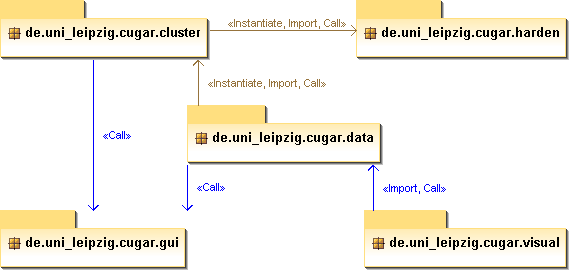
\includegraphics[width = 1\textwidth]{img/packageAll.png}
			\caption{Package cugar.*.} \label{fig:cvk.package}
		\end{figure}
		
	\subsubsection*{cugar.cluster}\label{sec:cvk.cluster}
		This package contains the adapter classes (\emph{ClusterAlgorithmBorderFlow}, \emph{ClusterAlgorithmKNN}, ...) for all supported clustering algorithms. 		
		Each of these adapter class is inherited from the abstract \emph{ClusterAlgorithm} class and implements 
		at least the abstract \emph{clustering} method and the \emph{getName} method as shown in figure \ref{fig:algos}. 
		These adapters are managed by the \emph{ClusterContext} class once they had loaded with a simple java class loader plugin system.
		You can add an algorithm via the plugin system without recompiling CUGAR   
		or you can add your algorithm by recoding the curarDemo method in entry point as shown in figure \ref{integration}.\\

		The example in figure \ref{integration} explicates how to implement and integrate an adapter (ClusterAlgorithmFoobar) for self-developed algorithm (Foobar). \\
		
		\begin{figure}[h!]
		The general is pretty simple, all you need to do is:\\
		
		1. Extend ClusterAlgorithm class by overriding the member String arrays to set new configuration options and implement 
		the abstract \emph{clustering} method and the \emph{getName} method.
		
		\lstinputlisting[linerange={10-30},language=Java]{codes.txt}%\caption{Example integration.}\label{alg:foobar}

		2(a). Integrate the adapter by modifying the \emph{cugar.gui.Main.cugarDemo} method which starts CUGAR.
		
		\lstinputlisting[linerange={1-6},language=Java]{codes.txt}%\caption{Modified cugarDemo method.}\label{main}	
		
		2(b). Integrate the adapter via the plugin system by creating a jar file, 
		which contains the ClusterAlgorithmFoobar.class file and depositing this jar in the plugin folder of CUGAR. 
		It is important that your class file is implemented in the \emph{cugar.cluster} package.
		\caption{Integration of a new algorithm}\label{integration}\end{figure} 
		
		In the 1st step of the integration, the four String parameters of the \emph{clustering} method comes from the member String arrays
		\emph{config\_A} ,..., \emph{config\_D} and can be used to provide possible paramaterizations of the novel algorithm. 
		For example, the implementation of kNN uses  \emph{config\_A = new String[]\{"k","1",...,"100"\}} for the parameter k. 
		It is important to notice that the first element of the array is the label shown in CUGAR for the parameter. 
		A user can choose the other elements of each array from a JComboBox in the application. 
		These are the values that are sent back to the  \emph{clustering} method as parameters so that they can be used for configurations. \\		
		The String array parameter \emph{seeds} gets all nodes that were added in Nodes table (figure \ref{fig:force}-left) to use as seeds.
		If no seeds added to the table, the seeds parameter will be  \emph{null} and the double parameter \emph{threshold} gets a value between 
		0 and 1 selected by the user from the threshold slider.\\		
		The return statement is a  \emph{prefuse.data.Table} with a specified column which
		holds the cluster data sets. The column name \emph{CLUSTER\_COLUMN\_NAME} and data type \emph{CLUSTER\_COLUMN\_NAME\_TYPE} are defined in  
		\emph{ClusterTableSettings} interface and are set to ``Cluster'' and TreeSet of String. 
		The  \emph{getTable()} method gets a valid table instance.\\
		The String member variable  \emph{filename} contains the path to a delimiter separated text file, the used separator get back by  \emph{getSeparator} method. \\
		It is possible to add more informations to the returned  \emph{prefuse.data.Table} instance, which will be displayed in the
		cluster table under the graph tab in the application.
		
		In 2(a). the first parameter of  \emph{addAlgorithm} method is the name of your algorithm shown in the application and has to be different from already existing names. 
		The second parameter is your algorithm instance. By starting the application all algorithm adapters will be instantiated.
		
		\begin{figure}[h!]
			\centering 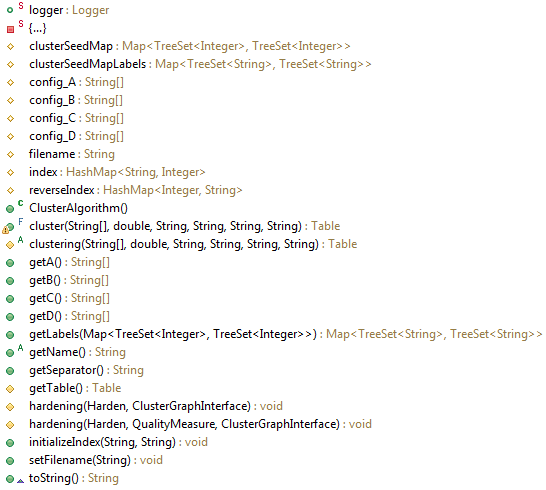
\includegraphics[width =1\textwidth]{img/clusterAlgorithmClass.png}
			\caption{Abstract ClusterAlgorithm class.} \label{fig:algos}
		\end{figure}

	\subsubsection*{cugar.data}
		This package provides a \emph{Model} class which has a instance of a \emph{ClusterContext} class to get 
		access to the current used algorithm (compare figure \ref{cvk.data}). Also, it provides 
		classes to read or generate data and the resulting graph is stored into a  \emph{prefuse.data.Graph} instance.		 

		The \emph{Model} class is the only class that needs to be accessed by external classes to read input data by means of the integrated 
		\emph{EdgeListGraphReader} or \emph{GraphMLReaderMod}, 
		to generate graphs by using the \emph{GraphGenerator} and to assign tasks to the currently chosen algorithm.

		\begin{figure}[h!]
			TODO ...
			%\centering 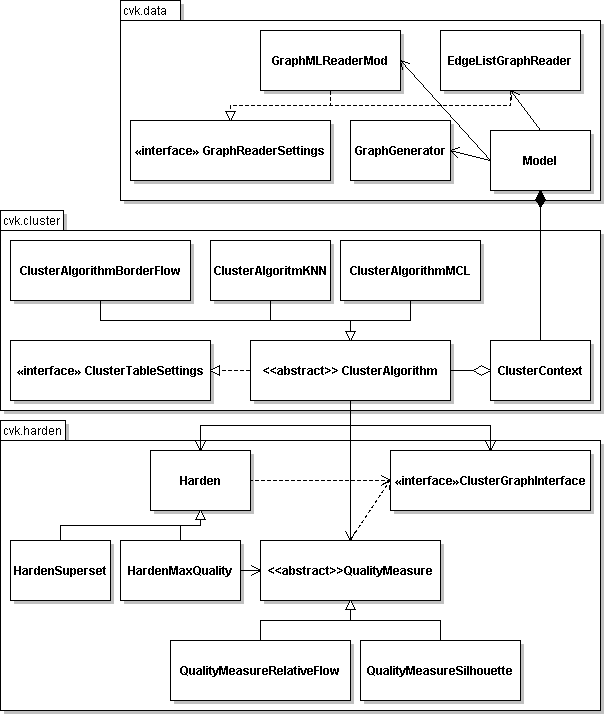
\includegraphics[width = 1\textwidth]{img/data.png}
			\caption{Package cugar.data, cugar.cluster and cugar.harden.} \label{cvk.data}
		\end{figure}
		
	\subsubsection*{cugar.harden}\label{sec:cvk.harden}
		\begin{figure}[ht!]
			\centering 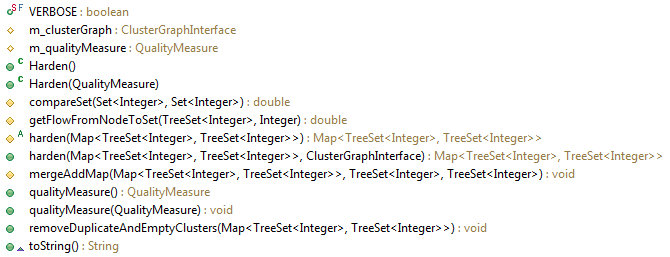
\includegraphics[width = 1\textwidth]{img/hardenClass.png}
			\caption{Abstract  \emph{Harden} class.} \label{fig:harden}
		\end{figure}

		This package contains the hardening strategies (described in section \ref{sec:harden}). 
		The hardening techniques implemented in this package can be used by all other algorithms implemented within CUGAR.\\
		
		To implement your own hardening strategy you can inherit from the abstract \emph{Harden} class and implement the abstract \emph{harden} method.
		The first parameter is a map of TreeSets that contains clusters as key and seeds as value. 
		The second parameter is a data structure of the graph that is used by the strategies. 
		The returned map is the hardening result.\\
		
		The \emph{ClusterAlgorithm} class described in \ref{sec:cvk.cluster} contains a member variable that can be used 
		as map for hardening and some other methods that supports develops by using their hardening strategy 
		(e.g., the hardening based on integer and the  \emph{ClusterAlgorithm} class has members for indexing and reverse indexing, this members  
		can be initialized with the \emph{initializeIndex} method).
		
	\subsubsection{The bf package}
		This package contains the BorderFlow and the k-Nearest Neighbors algorithms (described in section \ref{sec:algo}), 
		which were available from the beginning of this project on. 		
		The BorderFlow algorithm was developed independently from CUGAR and integrated in agreement with its main developer. 
	
	\subsection{Dependencies}
		\subsubsection{Prefuse}
			ClusterVisualizationKit uses the prefuse toolkit and therefore the prefuse library beta-20071021 has to be included in your lib folder. \\
			\url{http://prefuse.org}
		
		\subsubsection{Lucene}
			The prefuse toolkit supports a fast search with the Lucene search engine and we use it certainly.
			The library of Lucene search engine version 1.4.3 has to be included in your lib folder also. \\
			\url{http://lucene.apache.org/java/1\_4\_3}
		
		\subsubsection{Jung}
			The ``Java Universal Network/Graph Framework'' is used to generate random graphs.\\
			\url{http://jung.sourceforge.net}
		
		\subsection{Bugs }
			The application contain no critical bugs (i.e., bug that lead to a system failure) as far as we are awate. Still some minor bugs are still included in the library we utilize as listed in the subsequent section. Please do not hesitate to contact us if you have any helpful tips or comments on how to avoid these bugs. Furthermore, any feedback on unknown bugs will be greatly appreciated.

		\subsubsection*{java.lang.IllegalArgumentException}
			An IllegalArgumentException with an invalid row index is thrown after a clustering task sometimes.

\subsection{Change Log}
\subsubsection*{Version - beta 0.6 (25. January 2010)}
\begin{tabular}[ht]{ l  l }
Added & graph models\\
Added & some clustering algorithms\\
Added & clickable cluster table\\
Added & plugin system\\
Fixed & some small bugs\\
Fixed & manual
\end{tabular}
\subsubsection*{Version - beta 0.4 (9. August 2010)}
\begin{tabular}[ht]{ l  l }
Added & toolbar, java look and feel\\
Added & measurements\\
Added & mcl algorithm\\
Fixed & some small bugs
\end{tabular}

\subsubsection*{Version - beta 0.3 (7. July 2010)}
\begin{tabular}[ht]{ l  l }
Added & java doc to source \\
Added & graph generator for cliques and Erdos-Renyi\\
Added & harden for all algorithms\\
Added & split package cvk.data to package cvk.data.cluster\\
Fixed & covered draw of clusters \\
Fixed & ClusterAlgorithm class hierarchy\\
Fixed & some small bugs\\
\end{tabular}

\subsubsection*{Version - beta 0.2 (23. Jun 2010)}
\begin{tabular}[ht]{ l  l }
Added & image export\\
Added & graphml and delimiter file support\\
Added & load example graphs from menu\\
Added & log to file\\
Added & choice of a node from node list\\
Added & edge list in graph statistic\\
Added & knn algorithm \\
Fixed & ConcurrentModificationException\\
Fixed & some small bugs\\
\end{tabular}

\subsubsection*{Version - beta 0.1 (31. May 2010)}
First release.
\newpage
\bibliographystyle{plain}
\bibliography{lib}
\end{document}
